\chapter{Results}
\label{ch:results}

\section{Selection of feature selection technique}
Figure \ref{fig:selectionofselectiontech} shows the result of the comparison in terms of RMSE and Kendall Tau distance for feature selection techniques Chi-square, Information-Gain, Anova F-value, and Pearson correlation coefficient.

We see that the RMSE scores give most informative behaviour, and that the Pearson correlation coefficient outperforms the other feature selection techniques. So we use the only the RMSE and Pearson Correlation coefficient for the remaining research questions.

\begin{figure}[H]
    \centering
    \subfloat[\centering RMSE of four feature selection techniques for datasets Adult (blue), Mushroom (yellow), Optic (green), and the average value of all datasets (grey)]{{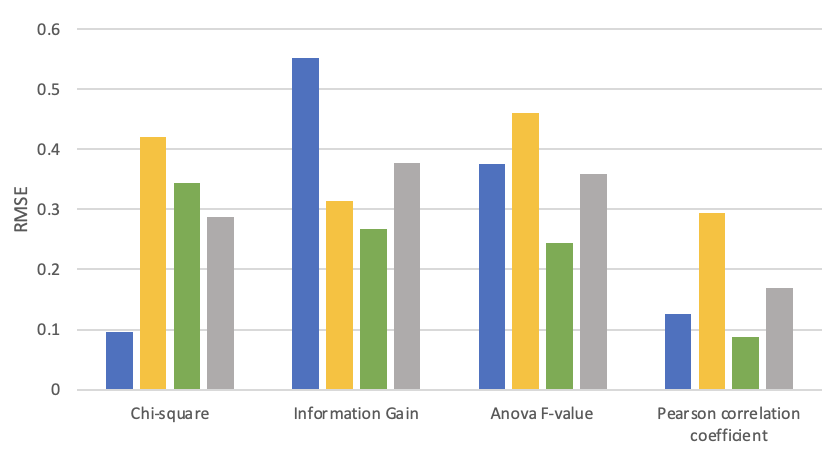
\includegraphics[width=6cm]{img/rq1figrmse.png} }}%
    \qquad
    \subfloat[\centering Kendall Tau distance of four feature selection techniques for datasets Adult (blue), Mushroom (yellow), Optic (green), and the average value of all datasets (grey)]{{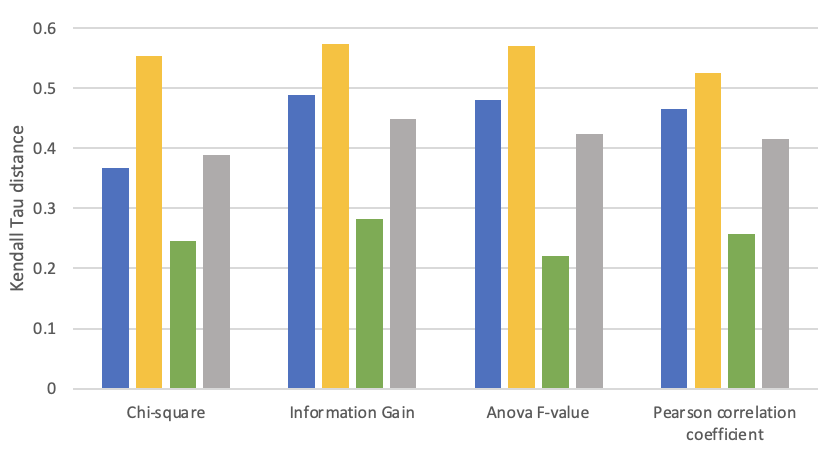
\includegraphics[width=6cm]{img/rq1figtaudist.png} }}%
    \caption{Heatmaps of Pearson correlation matrices for the Adult dataset.}
    \label{fig:selectionofselectiontech}
\end{figure}

\section{Features' correlation properties}
To gain insight into how the correlation between features is presered in anonymized datasets compared to the original dataset, we have depicted the heatmaps of feature's Pearson correlation scores in figures \ref{fig:heatmapsadult}, \ref{fig:heatmapsmushroom}, and \ref{fig:heatmapsoptic} for the Adult, Mushroom, and Optic datasets respectively. Only the first eleven relevant features are shown in the heatmap to improve visibility of the figure. The higher value (red) between two features shows that the associated features are more correlated, and the lower value (blue) shows less correlation. We observe that the scores in the correlation matrices for the differentially private datasets are a lot lower than in the original datasets. Therefore we include additional heatmaps with all self-correlations removed, this makes the heatmaps more visible because the range of the values in the heatmap is reduced.

From the heatmaps with self-correlations removed we can see that the correlation patterns have completely changed from the original dataset to the differentially private dataset. No correlation pattens from the original dataset could be identified in the differentially private dataset, meaning that values that were correlated before applying differential privacy are not correlated anymore after applying differential privacy.

\begin{figure}[H]
    \centering
    \subfloat[\centering Original Adult dataset]{{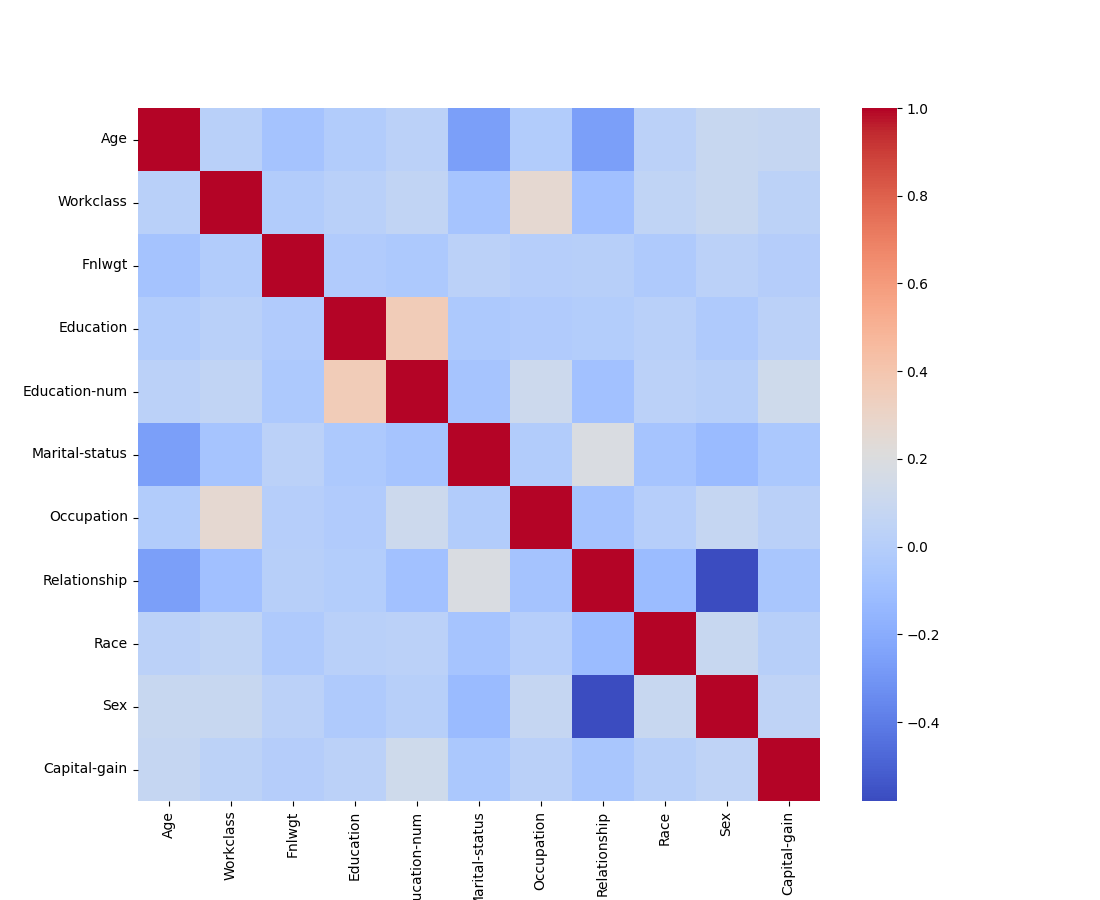
\includegraphics[width=4.7cm]{img/heatmapadultorig.png} }}%
    \qquad
    \subfloat[\centering Differentially private Adult dataset]{{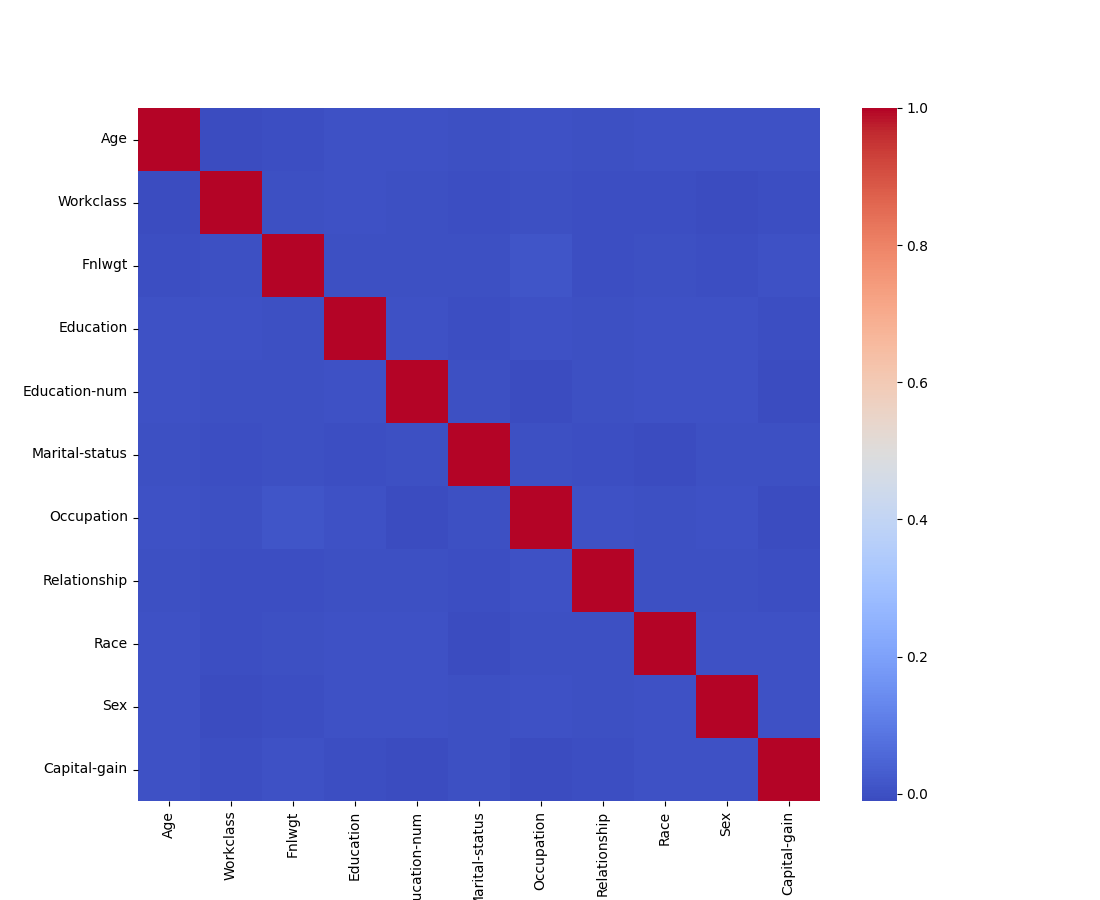
\includegraphics[width=4.7cm]{img/heatmapadultdp.png} }}%
    \qquad
    \subfloat[\centering Differentially private Adult dataset with self-correlation removed]{{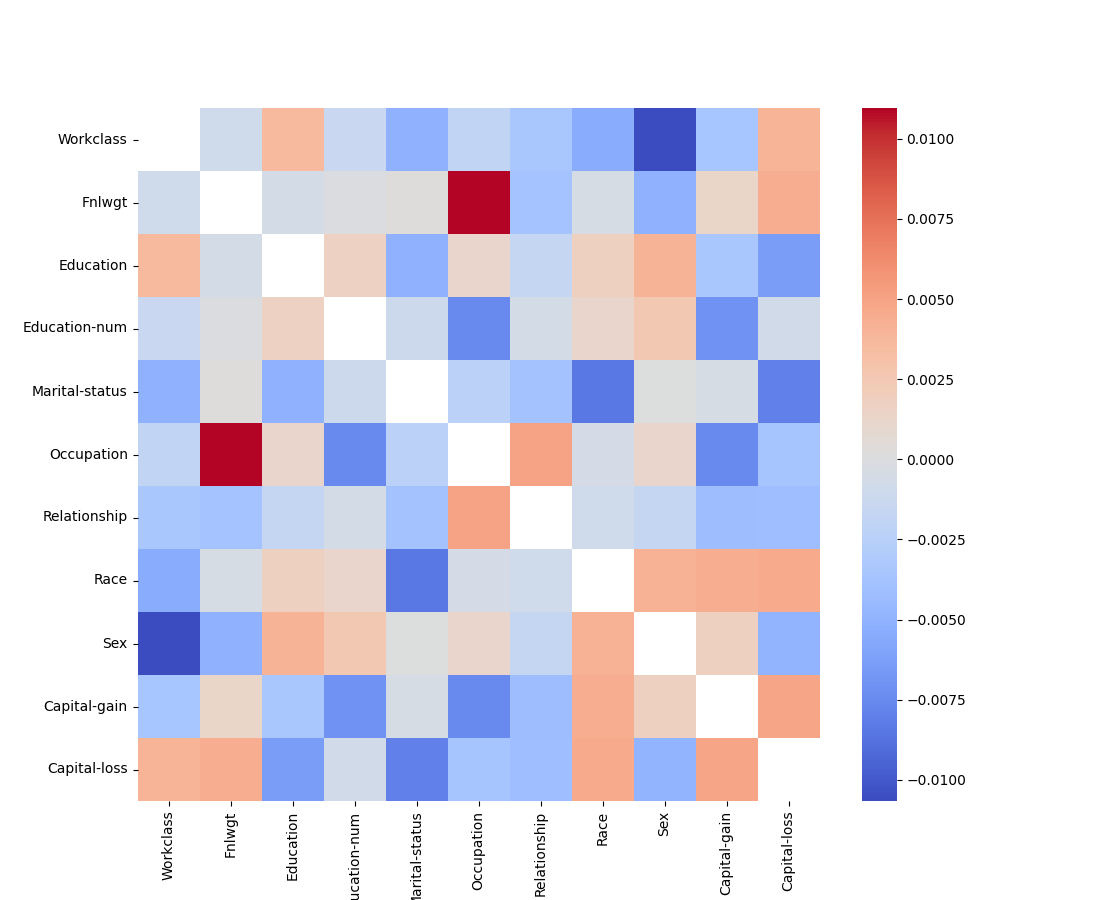
\includegraphics[width=4.7cm]{img/heatmapadultdp2.png} }}%
    \caption{Heatmaps of Pearson correlation matrices for the Adult dataset.}
    \label{fig:heatmapsadult}
\end{figure}

\begin{figure}[H]
    \centering
    \subfloat[\centering Original Mushroom dataset]{{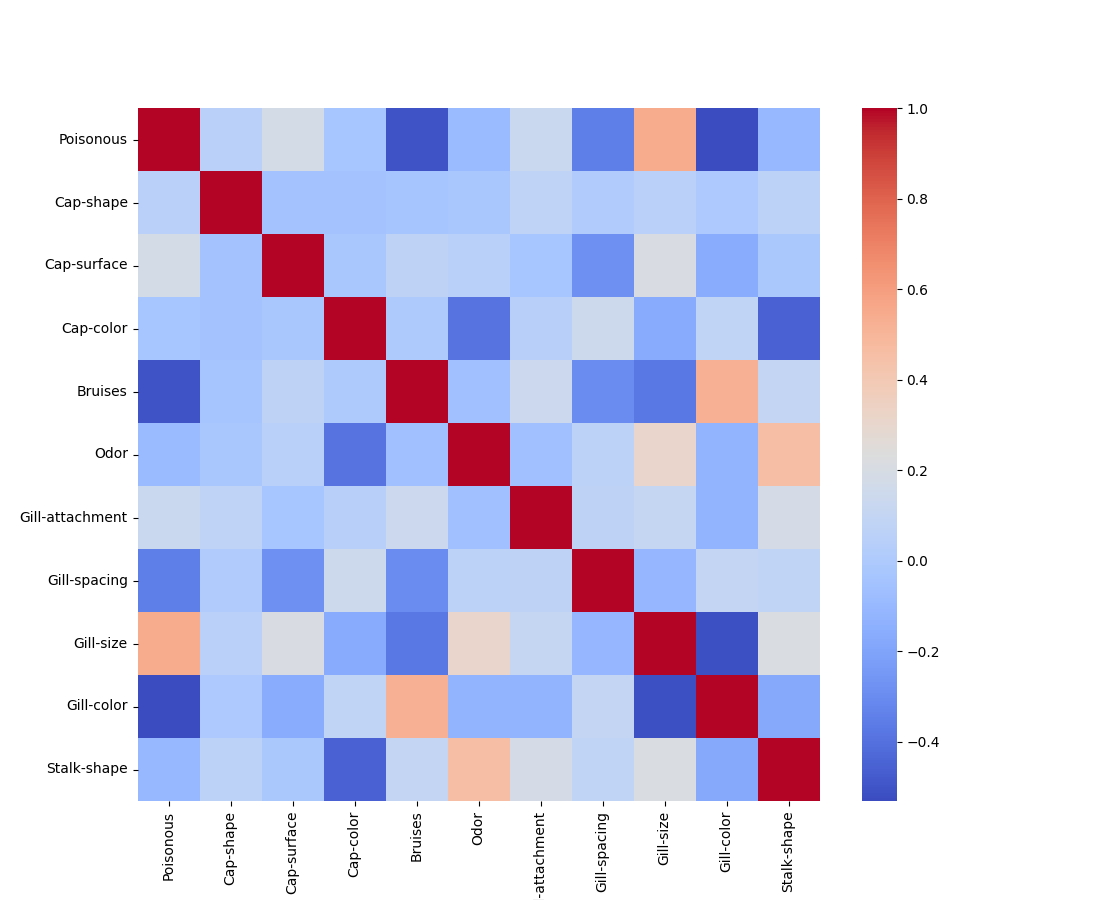
\includegraphics[width=4.7cm]{img/heatmapmushroomorig.png} }}%
    \qquad
    \subfloat[\centering Differentially private Mushroom dataset]{{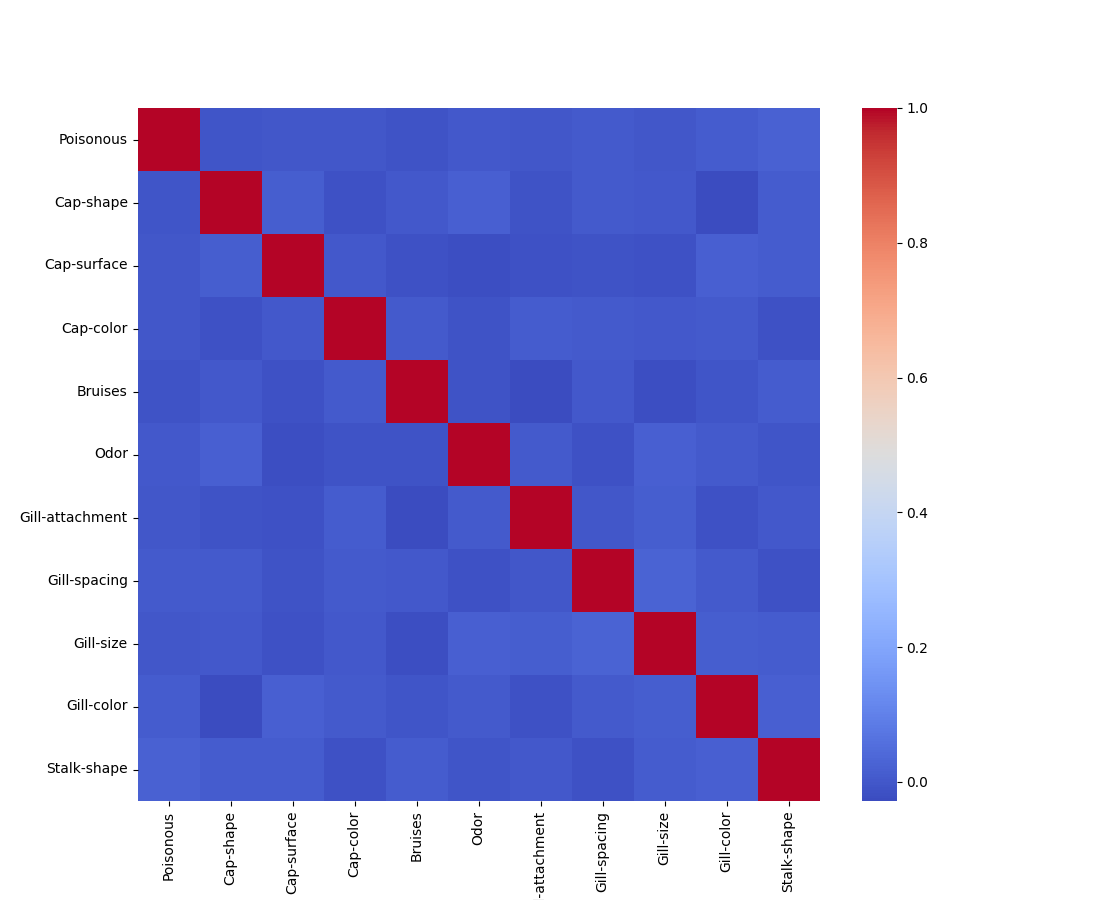
\includegraphics[width=4.7cm]{img/heatmapmushroomdp.png} }}%
    \qquad
    \subfloat[\centering Differentially private Mushroom dataset with self-correlation removed]{{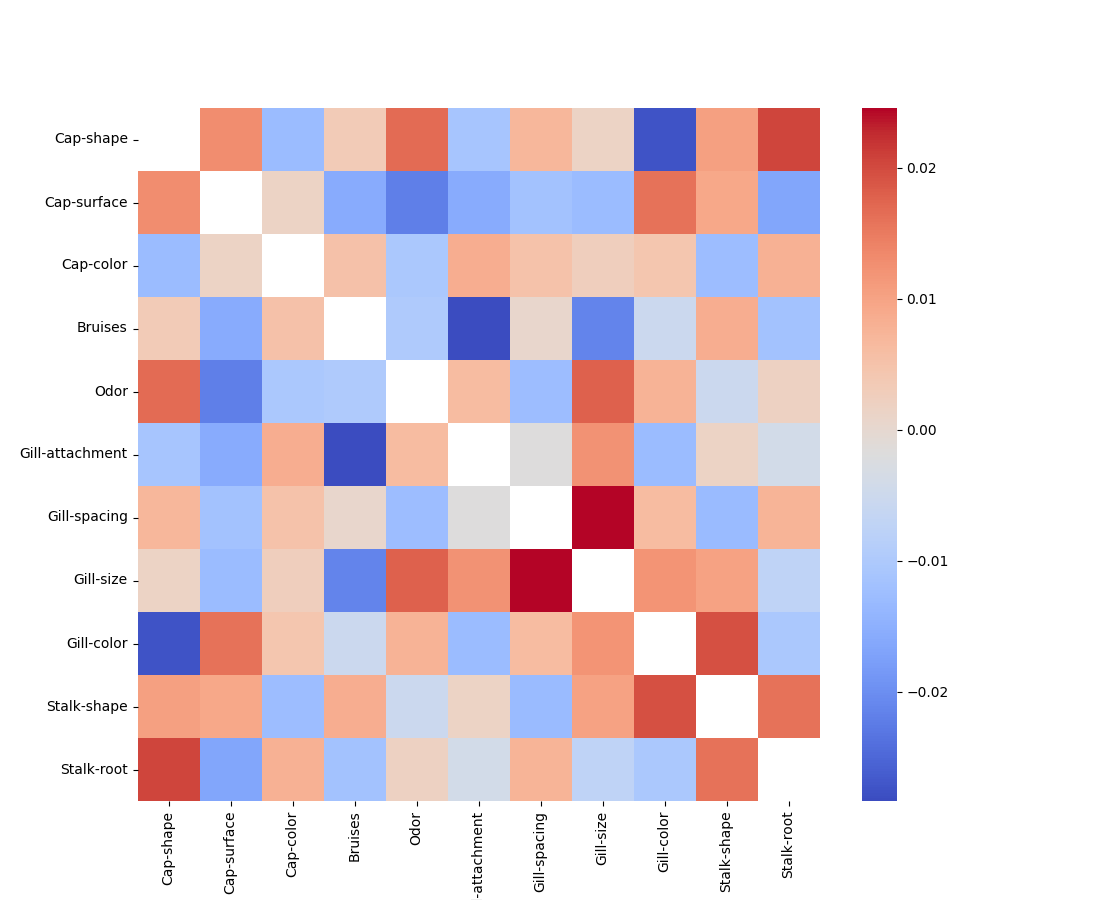
\includegraphics[width=4.7cm]{img/heatmapmushroomdp2.png} }}%
    \caption{Heatmaps of Pearson correlation matrices for the Mushroom dataset.}
    \label{fig:heatmapsmushroom}
\end{figure}

\begin{figure}[H]
    \centering
    \subfloat[\centering Original Optic dataset]{{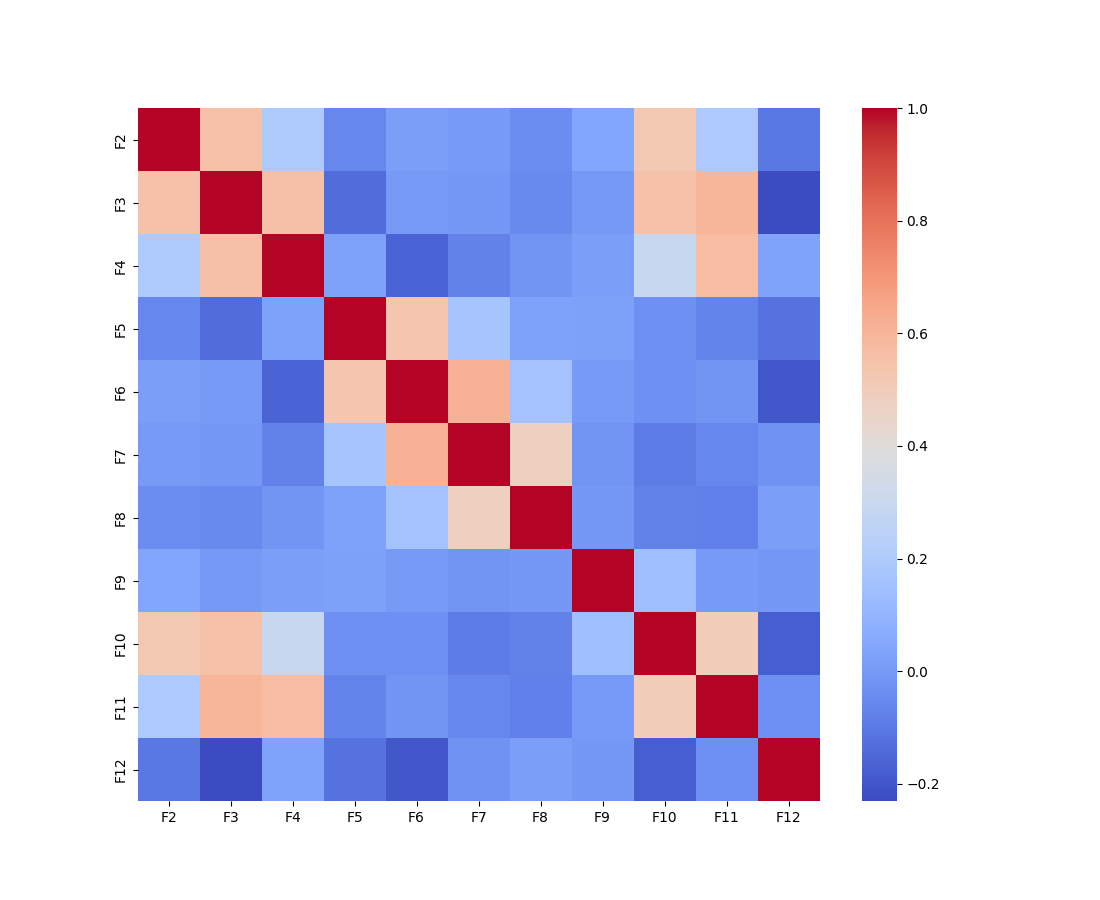
\includegraphics[width=4.7cm]{img/heatmapopticorig.png} }}%
    \qquad
    \subfloat[\centering Differentially private Optic dataset]{{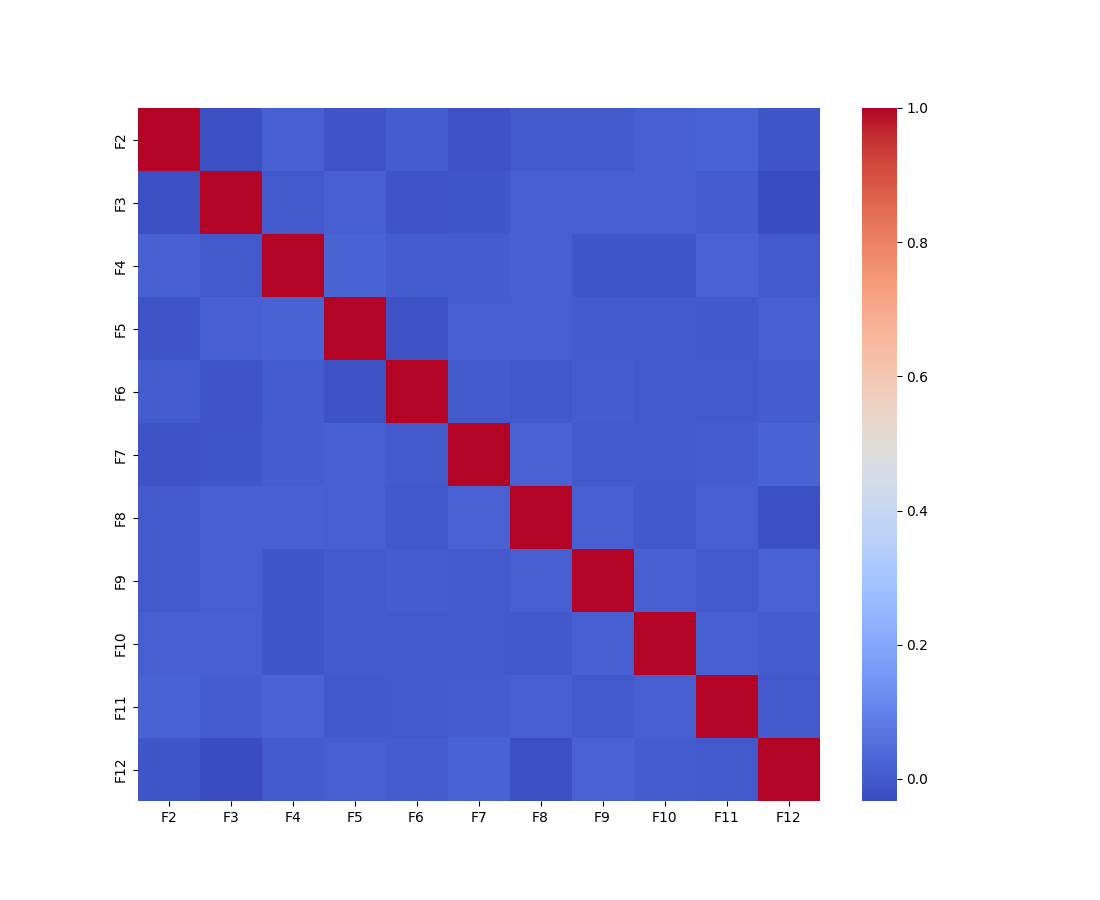
\includegraphics[width=4.7cm]{img/heatmapopticdp.png} }}%
    \qquad
    \subfloat[\centering Differentially private Optic dataset with self-correlation removed]{{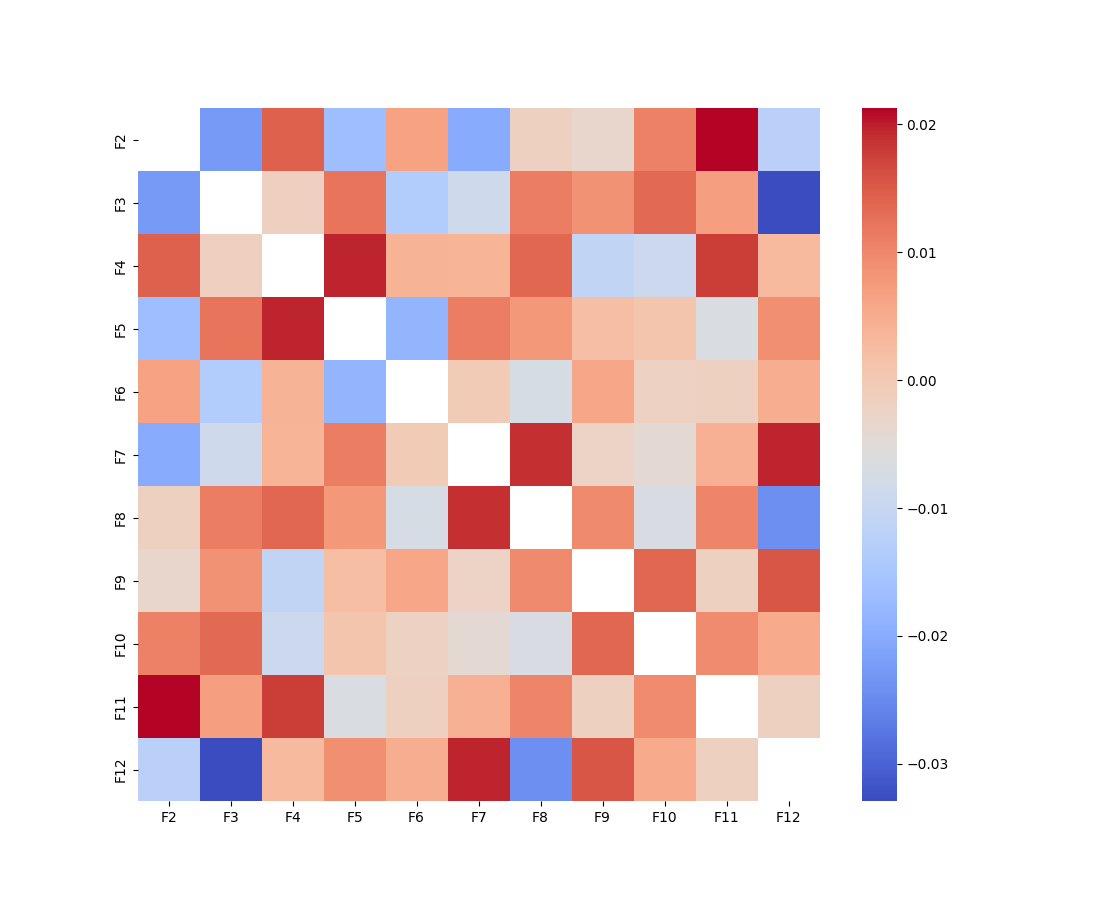
\includegraphics[width=4.7cm]{img/heatmapopticdp2.png} }}%
    \caption{Heatmaps of Pearson correlation matrices for the Optic dataset.}
    \label{fig:heatmapsoptic}
\end{figure}

\section{Impact of dataset properties}
The impact of dataset properties (dataset size, number of class labels, and number of features) on the RMSE between the Pearson correlation coefficient of the original dataset and the differentially private dataset is shown in figure \ref{fig:datasetparams}.

\begin{figure}[H]%
    \centering
    \subfloat[\centering Dataset size]{{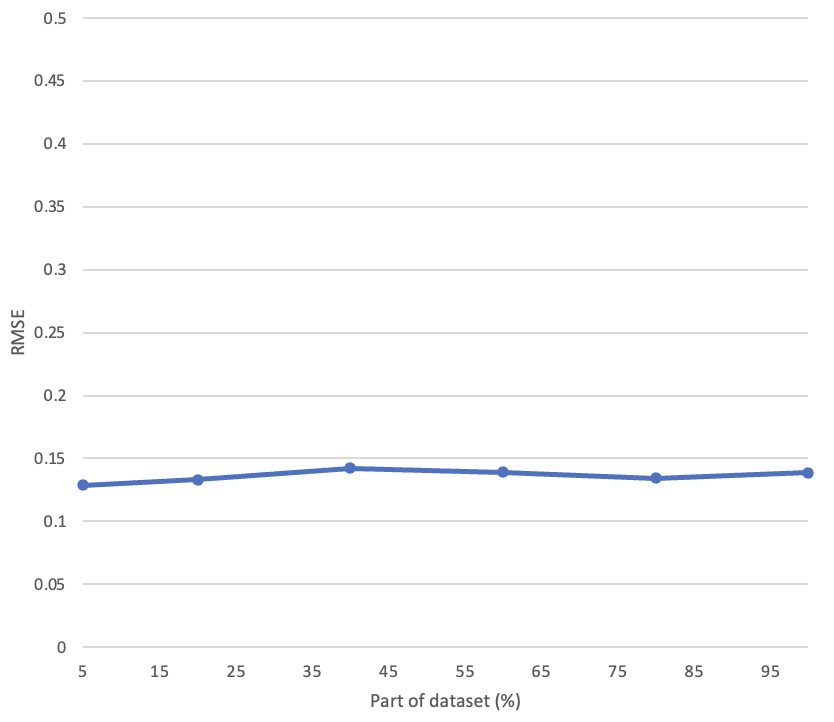
\includegraphics[width=4.5cm]{img/datasetsize.png} }}%
    \qquad
    \subfloat[\centering Number of class labels]{{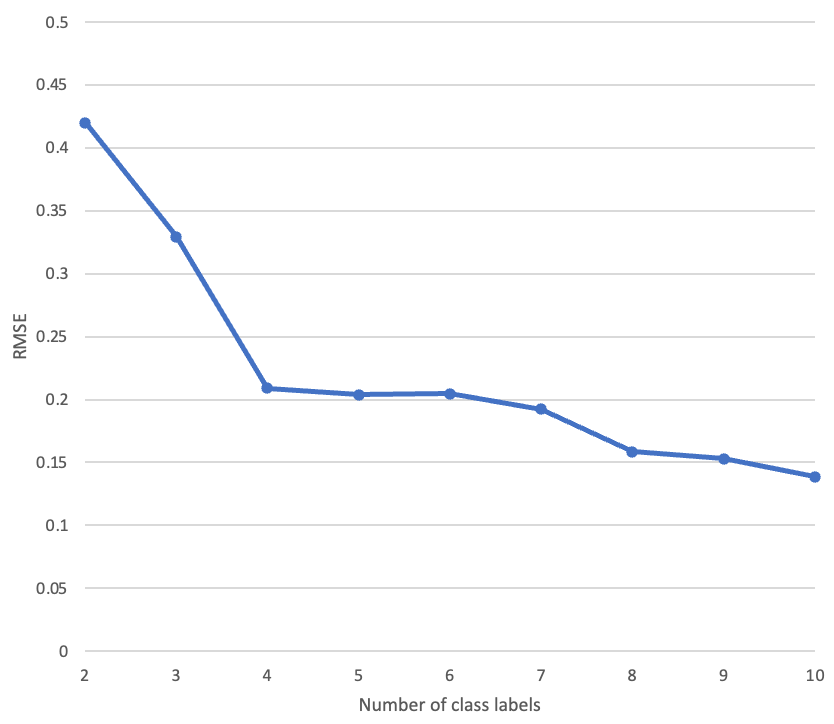
\includegraphics[width=4.5cm]{img/classlabels.png} }}%
    \qquad
    \subfloat[\centering Number of features]{{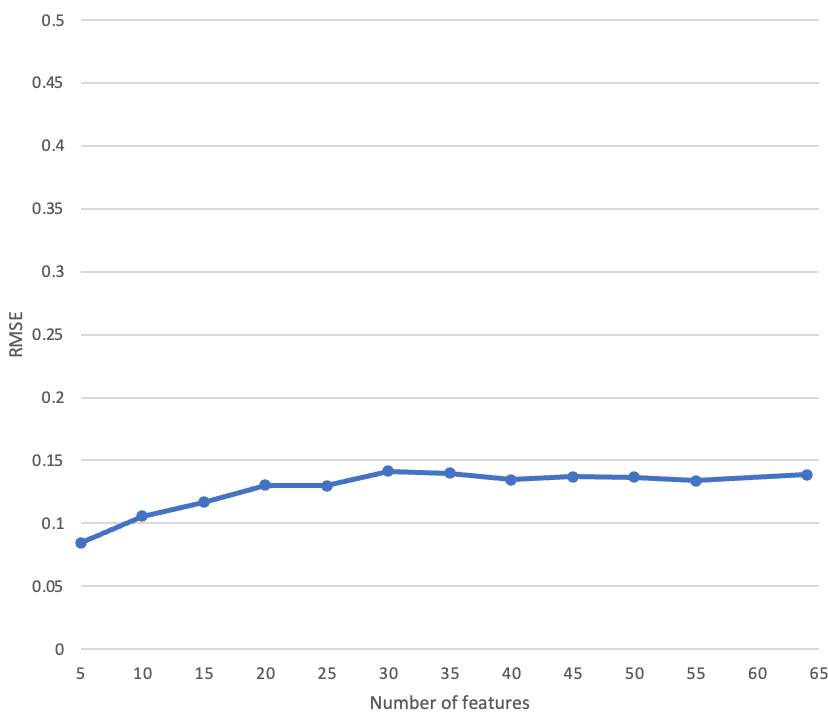
\includegraphics[width=4.5cm]{img/features.png} }}%
    \caption{The impact of varying the dataset parameters on the RMSE between the Pearson correlation coefficient of the original dataset and the differentially private dataset.}%
    \label{fig:datasetparams}%
\end{figure}

We observe that the dataset size does not have much impact on the Pearson correlation coefficient after applying differential privacy. 

However, the number of class labels has a large impact on the Pearson correlation coefficient. When the number of class labels is smaller than 4, the Pearson correlation coefficient is going down for larger numbers of class labels. From more than 4 class labels the Pearson correlation coefficient stabilizes and slightly goes down again for number of class labels higher than 6.

The number of features only affects the Pearson correlation coefficient for 30 features or less, but only slightly. With a number of features below 30 the RMSE between Pearson correlations is better than for 30 or more features. For 30 or more features the Pearson correlation coefficient is stable.\\

All observed Pearson correlation values for varying dataset parameters are within an acceptable range, except for the number of class labels below 4.

\section{Impact of differential privacy parameter}
The impact of the differential privacy parameter ($\epsilon$) on the RMSE between the Pearson correlation coefficient of the original dataset and the differentially private dataset is shown in figure \ref{fig:datasetparams}.

\begin{figure}[H]
    \centering
    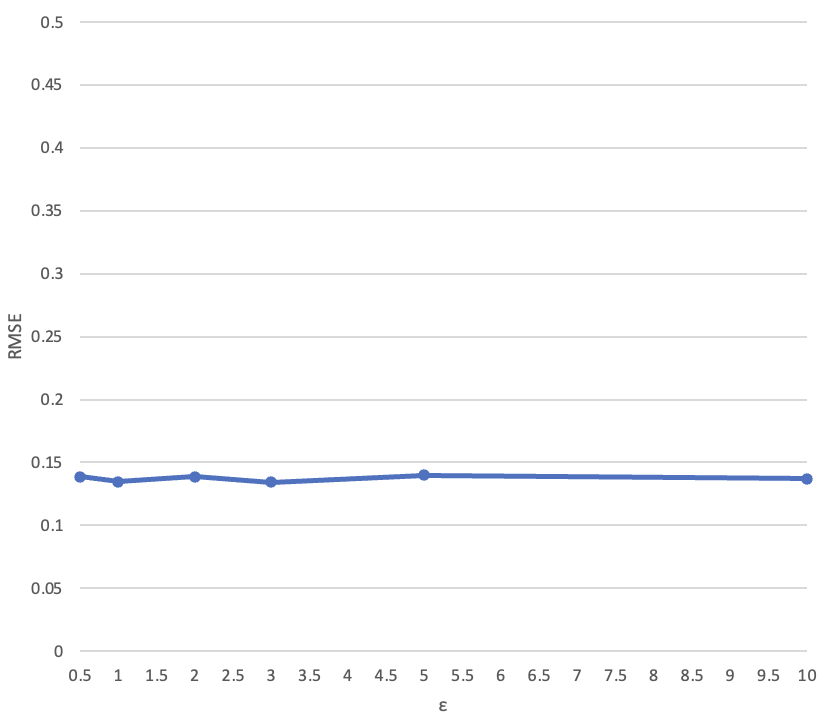
\includegraphics[width=5cm]{img/epsilon.png}
    \caption{The impact of varying the differential privacy parameter $\epsilon$ on the RMSE between the Pearson correlation coefficient of the original dataset and the differentially private dataset.}
    \label{fig:epsilonparam}
\end{figure}

The value of $\epsilon$ has no noticable effect on the Pearson correlation coefficient after applying differential privacy, its value is stable for all $\epsilon$ values. The value of $\epsilon$ might however influence other statistics that are beyond this research.

\section{Trained classifiers' impact}
Table 4.1 shows the classifier accuracy for Naive Bayes (NB), Decision Tree (DT), k-Nearest Neighbors (kNN), Random Forest (RF), Linear Regression (LR), and AdaBoost (AB) after keeping 20\% of the most relevant using Pearson correlation in original and differentially private datasets. The difference is shown in the last column.

All classifiers show similar differences and are positive close to 0, meaning that the performance of all classifiers is slightly worse when using the differentially private dataset than when using the original dataset. This small difference can be because of the small number of class labels in the Adult dataset.

\begin{table}[H]
\label{fig:classifiers}
\centering
\begin{tabular}{lllll}
Dataset                & Classifier & Original & Differentially private & diff. \\ \hline
\multirow{6}{*}{Adult} & NB         & 0.781    & 0.727                  & 0.054 \\
                       & DT         & 0.775    & 0.757                  & 0.018 \\
                       & kNN        & 0.771    & 0.724                  & 0.047 \\
                       & RF         & 0.769    & 0.747                  & 0.022 \\
                       & LR         & 0.781    & 0.755                  & 0.026 \\
                       & AB         & 0.784    & 0.749                  & 0.035 \\ \cline{2-5} 
                       & avg.       & 0.778    & 0.744                  & 0.034
\end{tabular}
\caption{Classifiers' accuracy for Naive Bayes (NB), Decision Tree (DT), k-Nearest Neighbors (kNN), Random Forest (RF), Linear Regression (LR), and AdaBoost (AB) after keeping 20\% of the most relevant using Pearson correlation in original and differentially private datasets.}
\end{table}

